% Black-and-white conceptual framework, drawn with TikZ.
% Compile: xelatex fig1_framework_tikz.tex
\documentclass[border=8pt]{standalone}

\usepackage{fontspec}
\setmainfont{Times New Roman}[
  BoldFont       = Times New Roman Bold,
  ItalicFont     = Times New Roman Italic,
  BoldItalicFont = Times New Roman Bold Italic]
\usepackage{tikz}
\usetikzlibrary{arrows.meta, calc}

\begin{document}
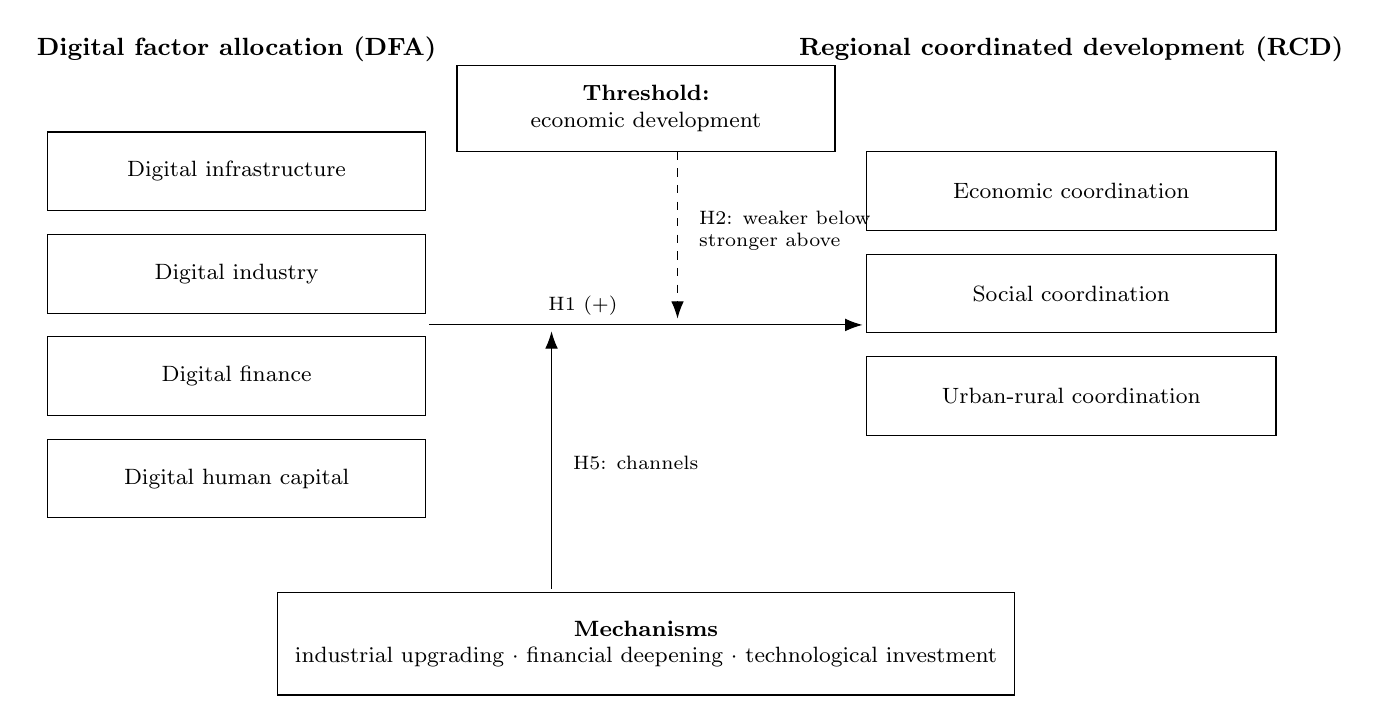
\begin{tikzpicture}[
  x=1cm, y=1cm,
  font=\footnotesize,
  box/.style   = {draw, thin, align=center, fill=white,
                  minimum height=10mm, inner sep=2.2mm},
  head/.style  = {font=\small\bfseries, align=center},
  arr/.style   = {-{Latex[length=2.2mm,width=1.6mm]}, thin},
  darr/.style  = {-{Latex[length=2.2mm,width=1.6mm]}, thin, dashed},
  note/.style  = {font=\scriptsize, align=left},
]

% ---------------------------------------------------------------- headers
\node[head] (lh) at (2.6,10.1) {Digital factor allocation (DFA)};
\node[head] (rh) at (13.2,10.1) {Regional coordinated development (RCD)};

% ---------------------------------------------------------------- left stack
\node[box, minimum width=4.8cm] (i1) at (2.6,8.55) {Digital infrastructure};
\node[box, minimum width=4.8cm] (i2) at (2.6,7.25) {Digital industry};
\node[box, minimum width=4.8cm] (i3) at (2.6,5.95) {Digital finance};
\node[box, minimum width=4.8cm] (i4) at (2.6,4.65) {Digital human capital};

% ---------------------------------------------------------------- right stack
\node[box, minimum width=5.2cm] (o1) at (13.2,8.30) {Economic coordination};
\node[box, minimum width=5.2cm] (o2) at (13.2,7.00) {Social coordination};
\node[box, minimum width=5.2cm] (o3) at (13.2,5.70) {Urban-rural coordination};

% ---------------------------------------------------------------- main path
\draw[arr] (5.05,6.60) -- (10.55,6.60);
\node[note] at (7.00,6.85) {H1 (+)};

% ---------------------------------------------------------------- moderator
\node[box, minimum width=4.8cm, minimum height=11mm] (thr) at (7.80,9.35)
  {\textbf{Threshold:}\\economic development};
\draw[darr] (8.20,8.80) -- (8.20,6.68);
\node[note, anchor=west] at (8.35,7.80) {H2: weaker below\\stronger above};

% ---------------------------------------------------------------- mechanisms
\node[box, minimum width=8.4cm, minimum height=13mm] (mech) at (7.80,2.55)
  {\textbf{Mechanisms}\\industrial upgrading \(\cdot\) financial deepening \(\cdot\) technological investment};
\draw[arr] (6.60,3.25) -- (6.60,6.52);
\node[note, anchor=west] at (6.75,4.85) {H5: channels};

\end{tikzpicture}
\end{document}
